\documentclass{article}
\usepackage{natbib}
\usepackage{color}
\usepackage[dvipsnames,svgnames*]{xcolor}
\usepackage{array}
\usepackage[colorlinks=TRUE, linkcolor=blue]{hyperref}
\usepackage[font=small,skip=5pt]{caption}
\usepackage[aboveskip=2pt]{subcaption}
\usepackage{graphicx}
\usepackage{amsmath}
\usepackage{amsthm}
\usepackage{amsfonts}
\usepackage{url}
\usepackage{ulem}
\usepackage{afterpage}
\usepackage{bbm}
\usepackage{hyperref}
\usepackage{Sweave}
\begin{document}
\Sconcordance{concordance:variationalwriteup.tex:variationalwriteup.Rnw:%
1 17 1 1 0 80 1}


We have the model

$$y_{t} = X^{'}_{t}\beta + \epsilon_{t},$$

where $Y$ is a $T \times 1$ random vector, $X$ is a $k \times T$ matrix of covariates, $\beta$ is a $k \times 1$ matrix of coefficients and $\epsilon_{t}$ is iid N$(0,\sigma^2).$

We are interested in the posterior density

$$p(\sigma^2, \beta | y) = \frac{p(y | \sigma^2, \beta)p(\sigma^2, \beta)}{p(y)}$$

Taking $p(\sigma^2, \beta) \propto \frac{1}{\sigma^2}$, 

\begin{eqnarray}
\label{joint}
p(\sigma^2, \beta | y) & \propto & \prod_{t=1}^{T} \frac{1}{\sigma} exp \left\{\frac{-1}{2 \sigma^2} (y_{t}-X^{'}_{t}\beta)^2 \right\} \frac{1}{\sigma^2} \nonumber \\
& = & \sigma^{-(T+2)} exp \left\{ \frac{-1}{2\sigma^2} \sum_{t=1}^{T} (y_{t}-X^{'}_{t}\beta)^2 \right\} \nonumber \\
& = & \sigma^{-(T+2)} exp \left\{ \frac{-1}{2\sigma^2}(T-k)\hat{\sigma}^2 \right\} exp \left\{ \frac{-1}{2\sigma^2} (\beta-\hat{\beta})'X'X(\beta-\hat{\beta})\right\} 
\end{eqnarray}

Where $\hat{\beta} = (X'X)^{-1}X'Y$, the OLS estimator of $\beta$ and $\hat{\sigma}^2 = (y-X\hat{\beta})'(Y-X\hat{\beta})/(T-k)$ is an unbiases estimator of $\sigma^2$.


We approximate $p(\beta, \sigma^2 | y)$ with $Q(\beta, \sigma^2) = Q(\beta)Q(\sigma^2)$, the factorisable distribution that minimises the Kullback - Leibler divergence between $p(\beta, \sigma^2 | y)$ and $Q(\beta, \sigma^2)$. It can be shown that the distributions $Q(\beta)$ and $Q(\sigma^2)$ that minimise this are: 

\begin{equation}
\label{Qb}
ln(Q(\beta)) = E_{\sigma^2}\left[ ln(y, \sigma^2, \beta))\right] + C
\end{equation}

and

\begin{equation}
\label{Qs}
ln(Q(\sigma^2)) = E_{\beta}\left[ ln(p(y, \sigma^2, \beta))\right] + C
\end{equation}

Substituting (\ref{joint}) into (\ref{Qb}) and ignoring the terms that do not depend on $\beta$, we get

$$ln(Q(\beta)) = E_{\sigma^2}\left[ \frac{-1}{2\sigma^2} (\beta-\hat{\beta})'X'X(\beta-\hat{\beta}) \right] + C$$.

Recognising the kernel of a normal distribution, we see that

$$Q(\beta) \sim N(\mu = \hat{\beta}, \lambda = (X'X)^{-1} E[\sigma^{-2}]^{-1})$$

Similarly substituting (\ref{joint}) into (\ref{Qs}) results in

\begin{eqnarray}
ln(Q(\sigma^2)) & = &  -(T+2)ln(\sigma) - \frac{1}{2\sigma^2} \left( (T-k)\hat{\sigma}^2 + E_{\beta}[(\beta-\hat{\beta})'X'X(\beta-\hat{\beta})] \right) + C \nonumber \\
& = & -(T+2)ln(\sigma) - \frac{1}{2\sigma^2} \left( (T-k)\hat{\sigma}^2 + tr(X'X Var(\beta)) \right) + C \nonumber
\end{eqnarray}

Recoginising the kernel of an inverse gamma distribution, we see that

$$Q(\sigma^2) \sim Inv.Gamma ( shape = (T+1)/2 = a, scale = \frac{(T-k)\hat{\sigma}^2 + tr(X'X \lambda)}{2} = b)$$

Therefore $1/\sigma^2 \sim Gamma(shape = a, rate = b)$ so $E[\sigma^{-2}] = a/b$, and substituting this into $\lambda$ gives us:


$$\lambda = (X'X)^{-1} b/a $$

and so
\begin{eqnarray}
b & = & \frac{(T-k)\hat{\sigma}^2 + tr(X'X (X'X)^{-1})b/a}{2} \nonumber \\
& = & \frac{(T-k)\hat{\sigma}^2}{2} + \frac{kb}{T+1} \nonumber \\
& = & \frac{(T-k)\hat{\sigma}^2}{2(1-k/(T+1))} \nonumber
\end{eqnarray}

Figure \ref{ex} shows the results of variational bayes compared to the exact posterior for the linear regression: $$y_{i} = b_{1} x_{1i} + b_{2} x_{2i} + \epsilon_{i}$$ 


\begin{figure}[htbp]
  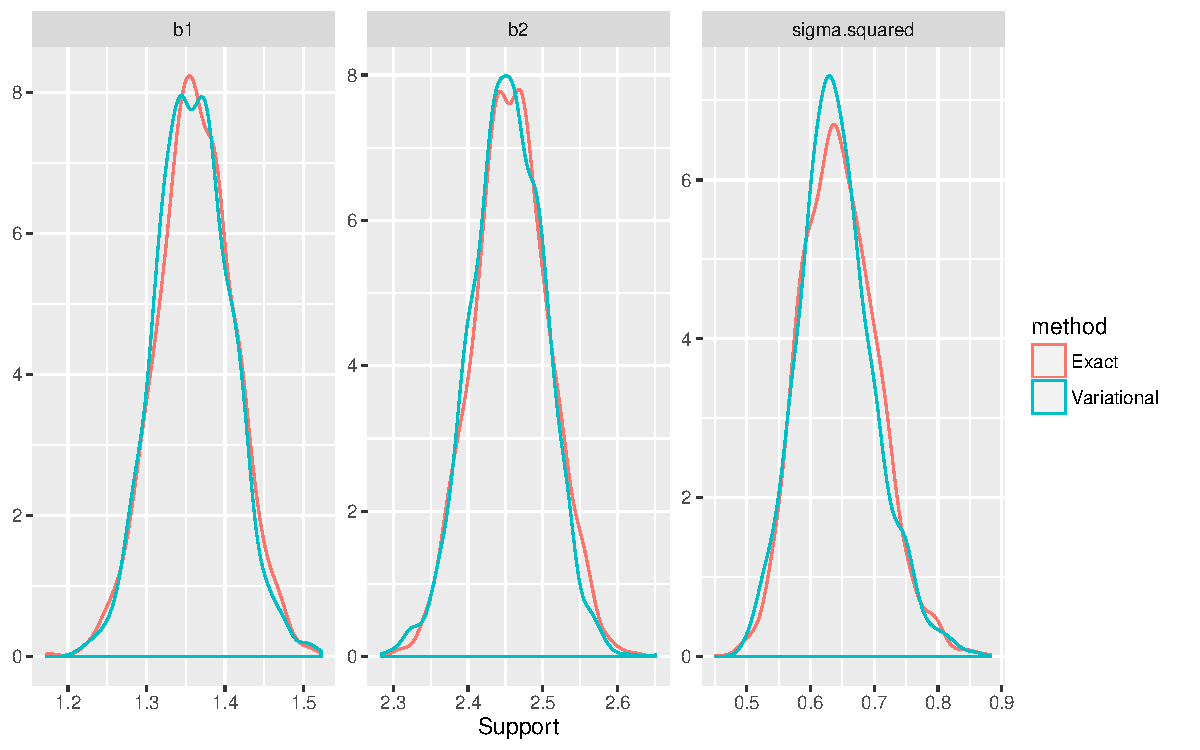
\includegraphics[height=8cm,keepaspectratio]{varbayes.pdf}
  \caption{Variational Bayes compared to the exact posterior. It took three iterations for the parameters to converge.}
  \label{ex}
\end{figure}


\end{document}
